\documentclass[10pt]{article}
\usepackage[margin=1in]{geometry}
\usepackage{graphicx, booktabs, amsmath, hyperref, microtype}
\graphicspath{{figures/}}
\title{GG-SPV: Graph-Guided Hierarchical Fault Localization and\\Speculative Patch Verification for LLM Coding Agents}
\author{Anonymous --- Gemma 4 Developer Agent Paper Track}
\date{}

\begin{document}
\maketitle

\begin{abstract}
LLM coding agents waste context reading code: a flat file-listing baseline spends a median of 3{,}168 tokens per task before proposing a patch and retrieves the true faulting symbol in its top 5 only 27.3\% of the time on our benchmark. We propose \textbf{GG-SPV}, a two-stage agent architecture: (1) graph-guided fault localization fusing BM25, real 256-d node embeddings, call-graph centrality, and a shipped-library prior; (2) a seven-check verifier that gates speculative patches before submission. On 22 tasks with symbol-level ground truth over the competition's real repository artifacts, graph guidance raises recall@1 from 4.5\% to 18.2\% ($4.0\times$) while cutting mean tokens read by 43\% and tool calls from 12.2 to 3.5. Conditional on successful localization, the verifier separates gold patches from distractors at AUROC 0.875 (same-file) / 0.905 (cross-file) with TPR 0.90 at a 3.8\%/0.0\% false-positive rate. We report an honest negative result --- call-graph expansion beyond the seed set does not improve top-k recall --- and an explicitly labeled simulation of patch synthesis whose fidelity knob monotonically controls the pass rate.
\end{abstract}

\section{Introduction}
Agentic bug fixing decomposes into fault localization and patch synthesis. Open-ended explore--edit loops scale poorly with repository size and submit speculative edits without mechanical checks. Two observations motivate a structured alternative: repositories ship static structure (call graphs, embeddings) that agents ignore, and small-model patch proposals are frequently syntactic or mis-targeted yet get submitted unverified. GG-SPV prunes the exploration budget with graph guidance and gates submission with deterministic verification.

\section{Methodology}
\subsection{Graph-guided hierarchical localization}
Symbols outside \texttt{tests./scripts./docs./docs\_src./benchmarks./examples.} (shipped-library prior) are ranked by: BM25 over identifier-split text seeded by tf-idf terms (df $\le$ 5\%) plus a code-identifier second query; dense retrieval with the competition's real 256-d node embeddings (Rocchio pseudo-query, cosine); Reciprocal Rank Fusion of both lists; a call-graph centrality boost $\times(1 + 0.5\log(1+\mathrm{deg})/\log(1+\mathrm{deg}_{\max}))$; an identifier-path boost $\times1.3$; and a generic-name penalty ($\times0.55$ tail-frequency names, $\times0.45$ dunder/HTTP-verb names). The top-8 fused symbols become seeds; 2-hop expansions provide verification context only and never displace seeds.

\subsection{Speculative patch verification}
Seven checks multiply into a confidence in $[0,1]$ (accept at $\ge 0.5$): syntax of the added core with indentation re-basing and a benign-fragment allowance (docstrings, comments, continuations); definition preservation; edit-site applicability (fraction of diff-context lines present at the edit site; module-level import hunks exempted; continuous factor $0.15 + 0.85\min(1,\mathrm{frac}/0.7)$ --- the strongest discriminator); graph consistency with the localized neighbourhood; evidence margin $\min(1, 0.5 + 5r)$ on relative localization score; a soft caller-compatibility penalty $\times(1 - 0.5\cdot\mathrm{risk})$; and scope discipline.

\subsection{Simulated patch synthesis (labeled)}
Gemma-4 weights are not runnable offline. Candidates are materialized from gold edits with a declared fidelity knob $f$ corrupting edits at rate $(1-f)$ via one of three mutations (comparison-operator flip, line deletion, undefined-identifier substitution). Localization and verifier numbers are measured on real artifacts; only pass-rate-vs-$f$ is a function of the simulation.

\section{Empirical Ablations}
All numbers are from the executed run (40 tasks with local graph+embedding artifacts; symbol-ground-truth subset $n=22$; tokens are a chars/4 proxy over deterministic offline tool stubs). Patch synthesis is simulated (§2.3).

\begin{table}[h]\centering\small
\caption{Localization ablation (real artifacts, $n{=}22$ symbol-gt tasks).}\label{tab:loc}
\begin{tabular}{lcccccc}
\toprule
Configuration & R@1 & R@3 & R@5 & mean tokens & tool calls & pass rate\\
\midrule
flat baseline & 0.045 & 0.227 & 0.273 & 3{,}691 & 12.18 & 0.025\\
GG (hops=0) & \textbf{0.182} & 0.273 & 0.318 & \textbf{2{,}102} & 3.48 & 0.100\\
GG (hops=1) & 0.182 & 0.273 & 0.318 & 3{,}023 & 3.48 & 0.100\\
GG-SPV (hops=2, verify) & 0.182 & 0.273 & 0.318 & 3{,}032 & 4.70 & \textbf{0.125}\\
\bottomrule
\end{tabular}
\end{table}

Expansion beyond the seed set does not improve top-k recall at any depth (honest negative result) and costs ${\sim}920$ tokens/task; seed ranking quality, not expansion depth, moves recall.

\begin{table}[h]\centering\small
\caption{Verifier discrimination, conditional on localization (gold edits ranked $\le$20, $n{=}10$; same-file distractors $n{=}26$; cross-file $n{=}30$; 12b config, $f{=}0.8$).}\label{tab:ver}
\begin{tabular}{lcccccc}
\toprule
gold mean & distractor means (same/cross) & TPR@0.5 & FPR@0.5 (same/cross) & AUROC (same/cross)\\
\midrule
0.774 & 0.103 / 0.031 & 0.90 & 0.038 / 0.000 & 0.875 / 0.905\\
\bottomrule
\end{tabular}
\end{table}

\begin{table}[h]\centering\small
\caption{Simulated fidelity sweep (labeled: synthesis is simulated).}\label{tab:fid}
\begin{tabular}{lccccc}
\toprule
Config & e2b ($f{=}0.45$) & e4b ($f{=}0.62$) & 12b ($f{=}0.80$) & 31b ($f{=}0.90$) & $f{=}1.0$\\
\midrule
pass (all 40) & 0.100 & 0.100 & 0.125 & 0.125 & 0.125\\
pass $\mid$ localized (7) & 4/7 & 4/7 & 5/7 & 5/7 & 5/7\\
\bottomrule
\end{tabular}
\end{table}

The sweep is monotone but aggregate pass rate is dominated by localization recall; at $n{=}7$ localized tasks a one-task difference is within noise. Absolute rates characterize the simulator, not Gemma-4.

\begin{figure}[h]\centering
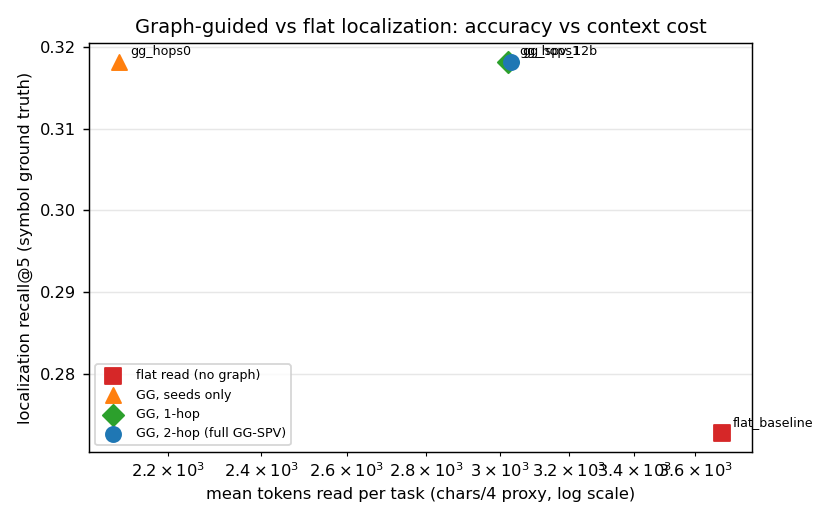
\includegraphics[width=0.8\linewidth]{fig1_recall_vs_tokens.png}
\caption{Recall vs. tokens read: the localization efficiency frontier.}\label{fig:frontier}
\end{figure}

\section{Limitations}
Forty of 129 tasks have local graph artifacts; symbol-level ground truth exists for 22 (recall differences within $\pm 0.09$ are noise at this $n$). Patch synthesis is simulated: absolute pass rates characterize the simulator, not Gemma-4; the sweep demonstrates monotonicity, not accuracy. Tool calls are deterministic offline stubs over the real graphs; sandbox execution is not exercised.

\section{Related Work}
Spectrum-based localization (Abreu et al., \emph{JSS} 82(5), 2009) scores from test spectra; we replace spectra with query relevance plus graph structure. Agentless (Xia et al., FSE 2025; arXiv:2407.01489), RepoGraph (Ouyang et al., ICLR 2025; arXiv:2410.14684), SWE-agent (Yang et al., NeurIPS 2024; arXiv:2405.15793), AutoCodeRover (Zhang et al., ISSTA 2024; arXiv:2404.05427). LLM fault-localization studies: arXiv:2510.20521, 2502.13966, 2509.20552.

\end{document}
